\chapter{Project Overview}
\href{https://www.youtube.com/watch?v=jvJtHYBX7sM}{Youtube}

In this project, you'll build a custom generative adversarial network to generate new images of faces.

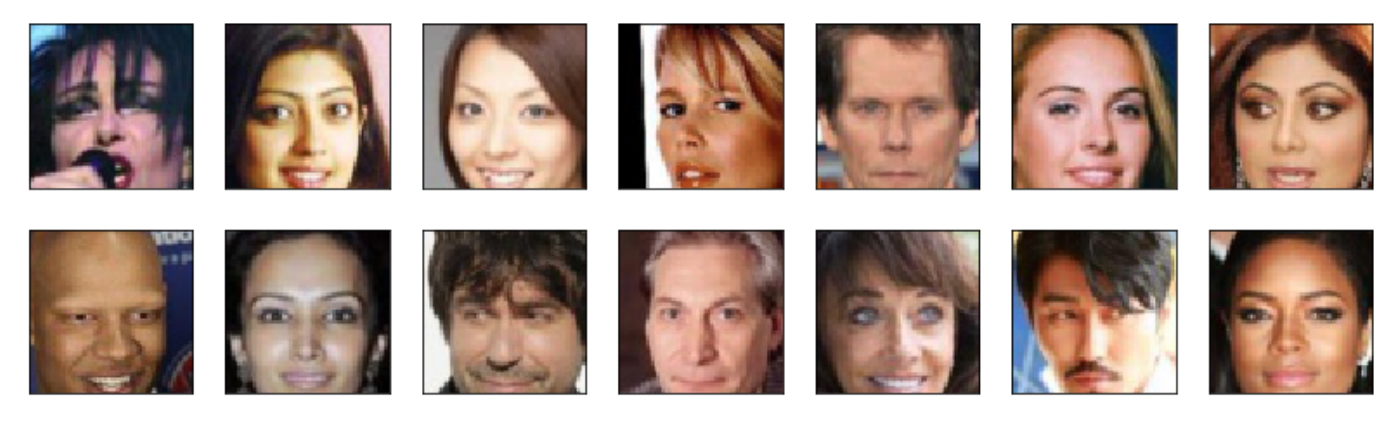
\includegraphics[width=1\linewidth]{img//genAdvNet/processed-face-data.png}
\captionof{figure}{Processed CelebA face data}

After training your model for a few epochs, you should be able to generate faces as seen below.
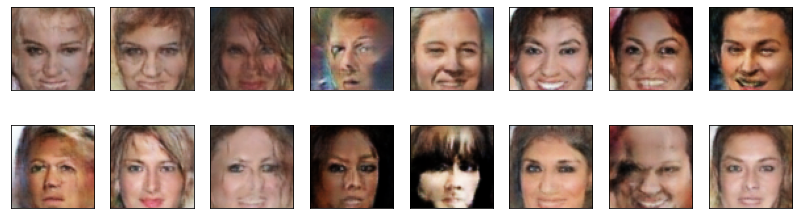
\includegraphics[width=1\linewidth]{img//genAdvNet/image-5.png}
\captionof{figure}{Generated faces}


\section{Getting the project files}

The project files are located in the Project Workspace and include the following files:

\begin{itemize}
    \item \textbf{\verb|dlnd_face_generation_starter.ipynb|}
    \item \textbf{\verb|README.md|}
    \item \textbf{\verb|requirements.txt|}
    \item \textbf{\verb|tests.py|}
    \item \textbf{\verb|processed-celeba-small.zip|}
\end{itemize}
We highly recommend using the Project Workspace to complete your project; however, if you choose to not use the workspace, you can download the project files from the Project Workspace.

\section{Instructions}

Open the notebook file, \verb|dlnd_face_generation_starter.ipynb| and follow the instructions. This project is organized as follows:

\begin{itemize}
    \item \textbf{Data Pipeline}: implement a data augmentation function and a custom dataset class to load the images and transform them.
    \item \textbf{Model Implementation}: build a custom generator and a custom discriminator to make your GAN
    \item \textbf{Loss Functions and Gradient Penalty}: decide on loss functions and whether you want to use gradient penalty or not.
    \item \textbf{Training Loop}: implement the training loop and decide on which strategy to use
\end{itemize}
Each section requires you to make design decisions based on the experience you have gathered in this course. Do not hesitate to come back to a section to improve your model or your data pipeline based on the results that you are getting.

Building a deep learning model is an iterative process, and it's especially true for GANs! Good luck!

\section{Submitting Your Project}

For this project you will need to submit one file – \verb|dlnd_face_generation.ipynb|.

The full project may be submitted in two ways:

\textbf{Project completed in Project Workspace:}

Your project may be submitted directly via the Project Workspace by pressing the \textbf{\verb|Submit|} button in the bottom right corner of the workspace.
\textbf{Project completed outside of Project Workspace:}

\begin{itemize}
    \item Your project may be submitted using the Project Submission page by pressing the \textbf{\verb|Submit Project|} button in the top right corner of the page and following those directions.
    \item You will need to create a zip file of the required project file and submit the zip file.
\end{itemize}
